\documentclass{Manual}


    \SetProyecto{Revista Universitaria}


% ------------------------------------ %

\begin{document}

    \frontmatter

\Portada
\Indices


% ------------------------------------ %

    \mainmatter


\chapter{Objetivos de la revista}

La presente revista estudiantil tiene como propósito fundamental establecer un espacio que vincule el trabajo realizado por los estudiantes con los procesos de publicación y comunicación científica.

Se plantean además los siguientes objetivos específicos:

\begin{enumerate}
    \item Introducir a los estudiantes en el proceso de publicación de artículos científicos, familiarizándolos con las etapas de redacción, edición, formato y envío, como parte de su formación profesional.

    \item Proveer a los alumnos de un producto académico adicional que pueda ser utilizado como material de apoyo en sus presentaciones y evaluaciones.

    \item Fomentar el interés y la motivación de los estudiantes en la publicación académica al ofrecerles la oportunidad de visualizar sus proyectos en un formato profesional, similar al de las revistas científicas consolidadas.

    \item Crear una biblioteca digital de los Proyectos Integradores desarrollados en la carrera, que sirva como fuente de consulta y referencia para futuras generaciones.

    \item Ampliar el alcance del repositorio mediante la posible inclusión de tesinas elaboradas por alumnos de sexto y décimo cuatrimestre durante sus estadías, ya sea como parte integrante de la revista o en una sección complementaria dentro del sitio web asociado.
\end{enumerate}
% \chapter{Justificación}

La creación de una revista científica interna para la carrera de Ingeniería en Biotecnología se fundamenta en la creciente evidencia sobre los beneficios de las publicaciones estudiantiles en la formación profesional. Diversos estudios han documentado que las revistas dirigidas por estudiantes constituyen un espacio formativo de alto valor pedagógico, al tiempo que contribuyen al ecosistema de investigación académica \citep{warren2025vital}.

En primer lugar, la experiencia de publicación permite a los estudiantes familiarizarse con el proceso editorial y de revisión por pares, competencias que tradicionalmente se adquieren hasta etapas avanzadas del posgrado. Como señalan Antony y colaboradores \citep{antony2025facilitating}, la participación en revistas estudiantiles facilita el aprendizaje del proceso de revisión por pares y promueve el desarrollo del pensamiento crítico, la alfabetización informacional y las habilidades de colaboración. De manera similar, la experiencia de la Nazarbayev University Graduate School of Education muestra que los estudiantes que participan como autores o revisores en revistas internas adquieren confianza para someter sus manuscritos a publicaciones internacionales y desarrollan una visión de la autoría como participación en una comunidad de práctica \citep{drybrough2025eight}.

En segundo lugar, la autenticidad de la audiencia constituye un factor determinante en la motivación y el desempeño de los estudiantes en tareas de escritura académica. Investigaciones en el ámbito de la formación docente han demostrado que escribir para una audiencia real—y no únicamente para la evaluación del docente—mejora significativamente la motivación, la autoeficacia y la percepción general de la escritura académica \citep{banegas2020learning}. Este hallazgo es consistente con lo reportado por la literatura sobre publicaciones estudiantiles, que indica que los estudiantes toman los proyectos más seriamente y aprenden más cuando el trabajo está dirigido a una audiencia externa en lugar de a una tarea de clase \citep{uaa2014undergraduate}. En el contexto específico de la escritura para publicación, Saputri y colaboradores \citep{saputri2023students} encontraron que la motivación inicial de los estudiantes noveles por publicar es alta, aunque puede fluctuar ante revisiones extensas, lo que subraya la importancia de contar con acompañamiento y procesos editoriales claros.

En tercer lugar, las revistas estudiantiles contribuyen a la construcción de la identidad académica de los participantes. Un estudio autoetnográfico sobre editores de revistas estudiantiles encontró que la experiencia editorial es relevante para el desarrollo de la identidad académica, particularmente en aspectos como el pensamiento reflexivo, la identidad autoral, la confianza y el aprendizaje a través de la crítica \citep{lujano2024exploring}. Este proceso es especialmente valioso en etapas tempranas de la formación, pues permite a los estudiantes visualizarse como productores de conocimiento y no solo como consumidores del mismo.

Las revistas científicas dirigidas por estudiantes han ganado reconocimiento como un elemento vital del ecosistema de investigación, con experiencias documentadas en diversas disciplinas como ciencias, medicina, derecho, políticas públicas y filosofía, entre otras \citep{warren2025vital}. El Student Journal Symposium, que en su segunda edición reunió a 73 estudiantes y profesionales representando 34 revistas estudiantiles de 28 universidades, evidencia el creciente interés y la consolidación de este tipo de iniciativas a nivel internacional \citep{warren2025vital}. Asimismo, la experiencia de la revista \textit{Current Issues in Education}, que celebra 25 años como publicación dirigida por estudiantes de posgrado, demuestra que estos proyectos pueden alcanzar sostenibilidad y generar impacto académico más allá de su institución de origen \citep{lujano2023special}.

Por otra parte, Huard \citep{huard2019showcase} distingue entre revistas de exhibición, que publican sin revisión por pares, y revistas selectivas, que implementan un proceso formal de revisión. La autora concluye que, si bien cualquier plataforma de publicación beneficia a los estudiantes, las revistas selectivas ofrecen beneficios acumulativos superiores tanto para los estudiantes—por la retroalimentación recibida y el prestigio de publicar en una revista de calidad—como para la institución y la comunidad académica en general. Este hallazgo respalda la intención de incorporar en la presente propuesta un proceso de revisión por pares realizado por alumnos de grados superiores.

Finalmente, la experiencia de la Washington University Journal of Undergraduate Research (WUJUR) ilustra cómo una revista estudiantil puede operar con un proceso estructurado y formal de revisión por pares, colaborar con departamentos universitarios y otras revistas, y ofrecer a los estudiantes una vía transparente y gratuita para la publicación de sus trabajos \citep{wujur2024mission}. Este modelo resulta pertinente para la presente propuesta, pues comparte el objetivo de visibilizar la producción estudiantil y fomentar la curiosidad y la excelencia académica.

En síntesis, la evidencia revisada sustenta que la implementación de una revista científica interna en la carrera de Ingeniería en Biotecnología no solo contribuiría a la formación de los estudiantes en competencias de comunicación científica y pensamiento crítico, sino que también fortalecería su identidad académica y motivación, al tiempo que generaría un acervo documental de valor para la comunidad educativa.
\chapter{Proceso de publicación}

\section{Periodos de publicación}

Dado que el principal objetivo de la revista es dar una mayor difusión de los trabajos realizados por los alumnos en la materia de Proyecto Integrador, la publicación de números nuevos se daría en base a la periodicidad de esta materia.

Por la organización del calendario escolar, esta materia tiene lugar en los periodos de Enero-Abril con 1 grupo, y en Mayo-Agosto con 2 grupos a la vez. Así pues, la publicación de nuevos números se realizaría en Abril y Agosto.

Dado que dos grupos presentarían proyectos en la publicación de Agosto, estaría a consideración si se publica un solo número con los trabajos de ambos grupos, o se divide en una ublicación por grupo. Asímismo, lo anterior se basa en que la revista se enfoque casi exclusivamente en los productos de la asignatura Proyecto Integrador, sin embargo, podrían existir más publicaciones si presenta el suficiente interés por parte de la comunidad estudiantil.

\section{Formatos de publicación}

La publicación de la revista sería en su mayor parte digital. Para esto se crearía una \textbf{\href{https://darahraccoon.github.io/BT_Magazine/}{página web}} en la cual se alojarían los números de la revista, así como los requisitos de envío y un enlace a la plantilla de Word/Docs.

Además de esto, se podría considerar realizar una impresión pequeña (3-4 ejemplares) para utilizarlas como recurso extra en las presentaciones de los proyectos.

\section{Tipos de publicaciones}

La revista tendría 2 tipos principales de artículos: Artículo de investigación y reviews.

Este tipo de trabajos son aquellos que los alumnos pueden llevar a cabo en la materia de Proyecto Integrador, por lo que solo sería necesario que lo especifiquen al momento de enviar su artículo.

Se propone para el primer número añadir publicaciones tipo Especial\footnote{El nombre puede cambiar}. Este se propone como un tipo de artículo que expanda la participación de los alumnos en la revista. Consistiría en artículos donde su formato sería más libre, aceptando artículos de divulgación, ensayos, producciones artísticas (poemas e ilustraciones, por ejemplo), etc., y donde las temáticas sean más variadas, tocando áreas de la biotecnología menos exploradas en la universidad, tales como las ciencias sociales, por ejemplo.

Los artículos de esta área los podrían enviar alumnos de cualquier cuatrimestre de manera voluntaria. Ya que estos trabajos no formarían parte de alguna asignatura, su proceso de revisión se establecería dependiendo del interés de los alumnos en publicar y en la disponibilidad de personas revisoras (docentes y/o alumnos). Asímismo, dependiendo del interés de los alumnos podría quedar como una sola categoría o segmentarse en varias.

\section{Proceso de envío}

Para familiarizar a los alumnos con el proceso de envío de artículos a una revista, se podría establecer un formato de envio el cual los alumnos deberán seguir para la publicación de sus artículos. El formato podría ser determinado en base a recomendaciones de docentes para que sea lo más similar posible al estándar académico.

A continuación se presentan algunos de los aspectos a definir en el formato, así como recomendaciones:

\begin{itemize}
    \item Tipo de archivo
        \subitem Google Docs o Word
    \item Características de la hoja
        \subitem Tamaño carta
        \subitem Márgenes de ~2.5cm en los 4 lados (por defecto en programas como Google Docs o Word)
        \subitem Sin encabezado ni pie de página
    \item Características de la tipografía
        \subitem Fuentes: Times New Roman o Arial
        \subitem Tamaño de fuente: 12pt
        \subitem Interlineado de 1.5
        \subitem Titulos a 16pt y en negritas
        \subitem Nombres científicos en itálica
    \item Figuras
        \subitem Enviar siempre archivos de imagen aparte
    \item Tablas
        \subitem De realizarse en hojas de cálculo (Excel, Sheets, etc.), adjuntar tales archivos
    \item Bibliografía
        \subitem Formato APA7
\end{itemize}


Tal como hacen algunas editoriales, se puede establecer también una plantilla que cumpla con los estándares de envío para facilitar la configuración del documento. A través de \textbf{\href{https://docs.google.com/document/d/1M7Ag4gmHuryCKiGC0duv6faO6SFfbrNe-7jA6rKuEZ4/edit?usp=sharing}{este enlace}} se presenta una propuesta de plantilla. 

\section{Revisión de artículos}

Dado que los artículos que se publicarán son producto de una materia con docente asignado, tal docente llevaría a cabo la revisión de los textos.

Aún así, podría existir un proceso de revisión por pares realizado por alumnos de mayor grado. Tal ejercicio podría expandir los beneficios académicos y pedagógicos de la revista al acercar a más alumnos al mundo de la academia y sus procesos.

\section{Proceso de maquetación}

La plantilla de LaTeX mediante la cual se maqueta la revista (\autoref{sec:plantilla_de_maquetación}) permite preparar los número unicamente copiando y pegando lo escrito por los alumnos en lugares determinados, por lo que la preparación de la revista sería algo sencillo que podría realizarse por una persona.
\chapter{Identidad gráfica}

Hasta ahora, las inspiraciones para la revista han sido \href{https://www.pentagram.com/work/scientific-american?rel=sector&rel-id=3}{un rediseño de la revista Scientific American}, la revista \href{https://www.frontiersin.org/journals/sustainability/articles/10.3389/frsus.2026.1818134/pdf}{Frontiers}, \href{https://www.sciencedirect.com/science/article/pii/S1198743X26000650/pdfft?pid=1-s2.0-S1198743X26000650-main.pdf}{Elsevier} y algunas ideas en \href{https://pin.it/3s68QTUbZ}{Pinterest}.

Si bien aún pueden realizarse mejoras, se esperará a recibir retroalimentación de docentes y alumnos para aplicarlas. Asímismo, en un futuro también se aceptarán recomendaciones de alumnos y docentes para mejorar el diseño de la revista.

\section{Paleta de colores}

La paleta de colores utilizada en la revista está inspirada en los colores institucionales de UPSIN. A continuación se listan los colores utilizados en la revista y las áreas en que se usa cada uno:

    \begin{figure}[H]
    \centering
    \begin{tikzpicture}
        \fill[Primario] (0,0) rectangle (5,5);
            \node[anchor=south,font=\sffamily\selectfont,white] at (2.5,0) {A};

        \fill[Acento] (5,0) rectangle (7.5,2.5);
            \node[anchor=south,font=\sffamily\selectfont,white] at (6.25,0) {C};
        \fill[Secundario] (5,2.5) rectangle (7.5,5);
            \node[anchor=south,font=\sffamily\selectfont,white] at (6.25,2.5) {B};

        \fill[Grey] (10,0) rectangle (12.5,2.5);
            \node[anchor=south,font=\sffamily\selectfont,black] at (11.25,0) {E}; 
        \fill[Complemento] (10,2.5) rectangle (12.5,5);
            \node[anchor=south,font=\sffamily\selectfont,black] at (11.25,2.5) {D};
    \end{tikzpicture}
    \rule{\linewidth}{0.2pt}
    \caption{Paleta de colores}
    \label{fig:paleta_de_colores}
\end{figure}

        \definecolor{Primario}{RGB}{9,60,113}
        \definecolor{Secundario}{RGB}{0,160,224}
        \definecolor{Acento}{RGB}{138,222,255}
        \definecolor{Complemento}{RGB}{245,230,80}

\begin{itemize}
    \item Color principal (A) - RGB(9,60,113)
        \subitem Contador de tablas y figuras (Tabla X, Figura X)
        \subitem Color de fondo para encabezado en tablas a una columna
        \subitem Enlaces externos
    \item Color secundario (B) - RGB(0,160,224)
        \subitem Enlaces internos (citas, figuras y tablas)
    \item Color de acento (C) - RGB(138,222,255)
    \item Color de complemento (D) - RGB(245,230,80)
    \item Gris (E) - RGB(242,242,242)
        \subitem Color de fondo para filas en tablas (intercalado con blanco)
\end{itemize}

\section{Tipografías}

Se estarían utilizando 2 tipografías: Red Hat Display y Crimson Pro. Cada una sería utilizada en diferentes  áreas.

La tipografía Red Hat Display (\autoref{fig:tipografía_red_hat_display}) sería utilizada para titulos y encabezados, variando y combinando su estilo y peso (negrita, normal e itálica) para cada nivel de titulo o encabezado. También se estaría utilizando para los contadores de figuras y tablas (Tabla X, Figura X).

    \vspace{1em}
\begin{figure}[H]
    \centering
    {\sffamily\LARGE\selectfont \textbf{AaBbCc} \quad  AaBbCc \quad \textit{AaBbCc}}
    \vspace{1em}
    \textcolor{Primario}{\rule{\linewidth}{0.2pt}}
    \vspace*{-2em}
    \caption{Tipografía Red Hat Display (Negritas, normal e itálica)}
    \label{fig:tipografía_red_hat_display}
\end{figure}

Por otro lado, la tipografía Crimson Pro (\autoref{fig:tipografía_crimson_pro}) sería utilizada para el texto principal, así como descripciones de tablas y figuras.

    \vspace{1em}
\begin{figure}[H]
    \centering
    {\LARGE\selectfont \textbf{AaBbCc} \quad  AaBbCc \quad \textit{AaBbCc}}
    \vspace{1em}
    \textcolor{Primario}{\rule{\linewidth}{0.2pt}}
    \vspace*{-2em}
    \caption{Tipografía Crimson Pro (Negritas, normal e itálica)}
    \label{fig:tipografía_crimson_pro}
\end{figure}


Para el texto general se utilizará un tamaño de 12pt. Para los encabezados de distintos niveles se utilizarán los siguientes tamaños:

\begin{itemize}
    \item 18pt en negritas 
    \item 16pt en negritas
    \item 14pt en itálica
\end{itemize}

\section{Presentación de tablas y figuras}

\subsection{Tablas}

Los encabezados de las tablas tendrán Red Had Display como tipografía, mientras que el resto de la tabla (cuerpo y notas a pie) mantendrán Crimson Pro como tipografía.

El color de las filas del cuerpo alternará entre blanco y gris. En el caso de los encabezados estos podrán utilizar el color primario (azul oscuro, \autoref{tab:ejemplo_tabla_azul}) o blanco como color de fondo (\autoref{tab:ejemplo_tabla_blanco}).

    \newpage

\begin{multicols}{2}

\begin{table}[H]

\caption{Ejemplo de tabla con encabezados color azul}
\label{tab:ejemplo_tabla_azul}

\begin{threeparttable}

{\small\setstretch{1.35}\rowcolors{1}{Grey}{White}

\begin{tabular}{M{0.4\linewidth}M{0.4\linewidth}}\hline
    
    \sffamily\bfseries\cellcolor{Primario}\textcolor{White}{Encabezado 1} & \sffamily\bfseries\cellcolor{Primario}\textcolor{White}{Encabezado 2} \\ \hline
    
    Dato 1 & Dato 2\tnote{1} \\
    Dato 3 & Dato 4 \\
    Dato 5 & Dato 6 \\
    Dato 7 & Dato 8 \\

    \hline
\end{tabular}

}

\begin{tablenotes}\tiny % ex: \tnote{1} ... \item[1]
    \item[1] Ejemplo de nota a pie de tabla
\end{tablenotes}

\end{threeparttable}
\end{table}



\begin{table}[H]

\caption{Ejemplo de tabla con encabezados color blanco}
\label{tab:ejemplo_tabla_blanco}

\begin{threeparttable}

{\small\setstretch{1.35}\rowcolors{1}{Grey}{White}

\begin{tabular}{M{0.4\linewidth}M{0.4\linewidth}}\hline
    
    \sffamily\bfseries\cellcolor{White}\textcolor{Primario}{Encabezado 1} & \sffamily\bfseries\cellcolor{White}\textcolor{Primario}{Encabezado 1} \\ \hline
    
    Dato 1 & Dato 2\tnote{1} \\
    Dato 3 & Dato 4 \\
    Dato 5 & Dato 6 \\
    Dato 7 & Dato 8 \\

    \hline
\end{tabular}

}

\begin{tablenotes}\tiny % ex: \tnote{1} ... \item[1]
    \item[1] Ejemplo de nota a pie de tabla
\end{tablenotes}

\end{threeparttable}
\end{table}

\end{multicols}

\subsection{Figuras}

En el caso de las figuras se respetará el diseño de los autores originales. Se usará una linea azul oscuro para separar la figura de la descripción.

\begin{figure}[H]
    \centering
    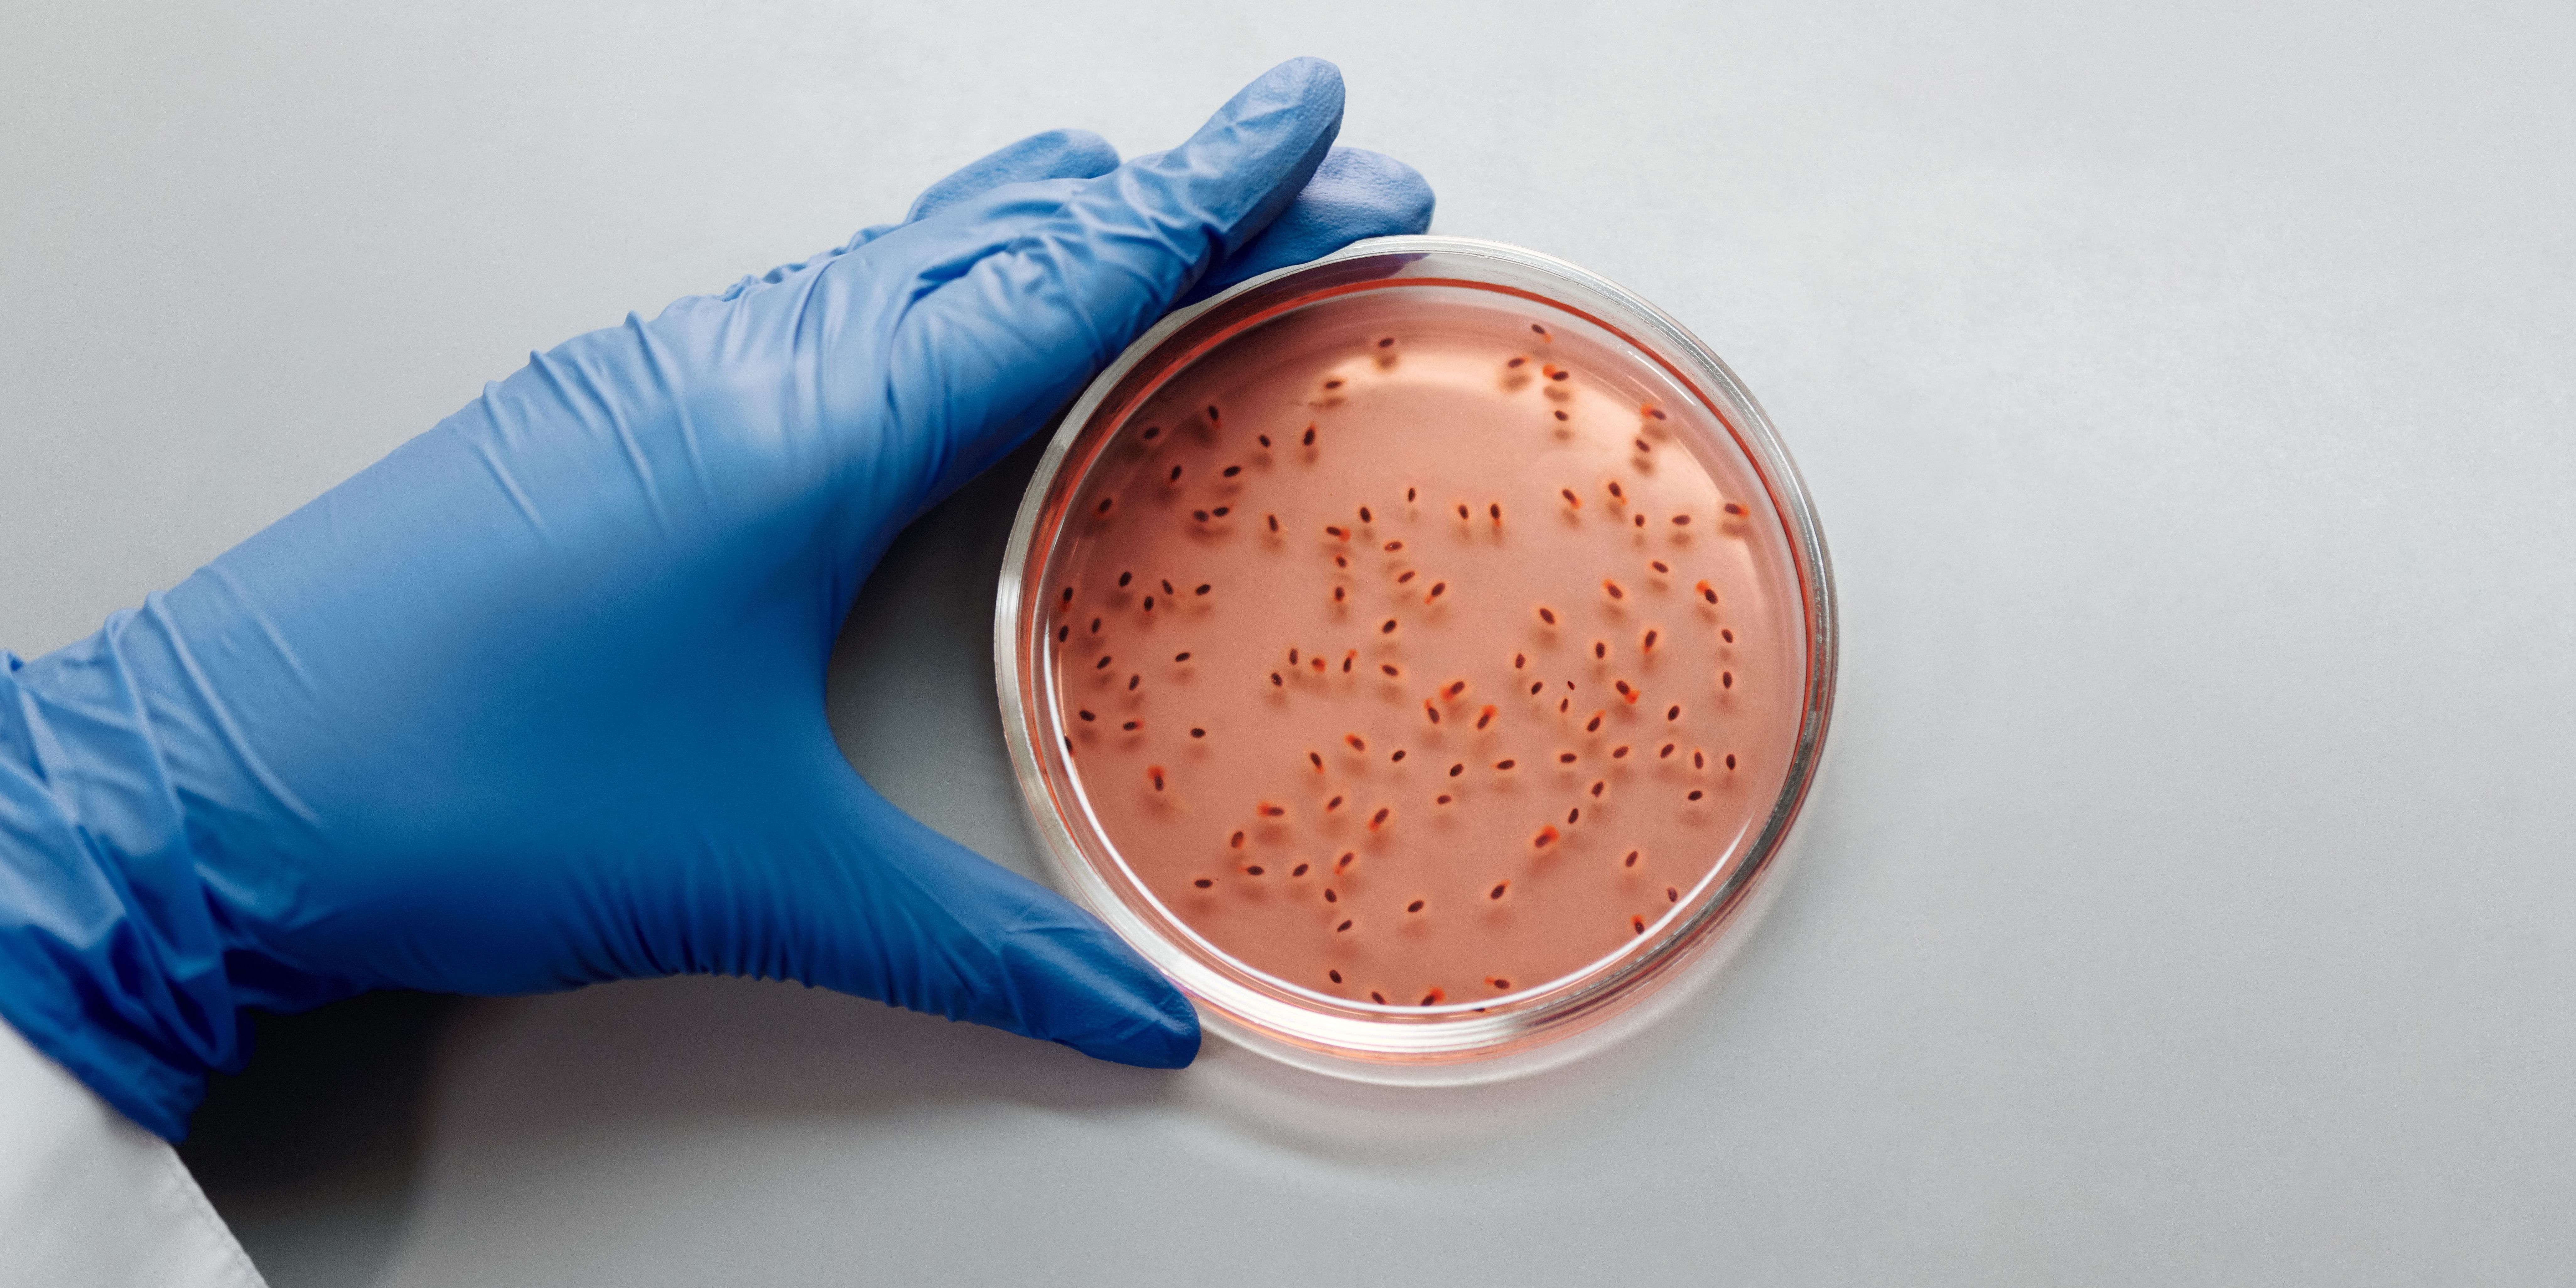
\includegraphics[width=0.85\linewidth]{fig:ejemplo_figura}
    \textcolor{Primario}{\rule{\linewidth}{0.2pt}}
    \caption{Ejemplo de figura}
    \label{fig:ejemplo_figura}
\end{figure}


% ------------------------------------ %
    
% \bibliography{Main}\addcontentsline{toc}{chapter}{Bibliografía}
    
    \appendix
    
\chapter{Plantilla de maquetación en LaTeX}\label{sec:plantilla_de_maquetación}
    \begin{verbatim}
        % USO: \SetTituloActual{Titulo corto del artículo}
        \SetTituloActual{}

        % USO: \Inicio{Tipo de artículo}{Título del artículo}}{Autores}   
        \Inicio{}{}{}

        %% Tipos de artículo (En mayúsculas):
           % ARTÍCULO DE INVESTIGACIÓN
           % REVIEW
           % ESPECIAL

        % USO: \Resumen{Texto del resumen}{Palabras clave}
        \Resumen{}{}

            \begin{multicols}{2} % Establece el formato de 2 columnas
            
        % Pegar el texto de los alumnos en las secciones correspondientes
        
        \section{Introducción}
        \section{Materiales y métodos}
        \section{Resultados}
        \section{Discusión}
        \section{Conclusión}

        % Inserta la bibliografía del artículo con estilo APA7
        % La X se cambia por el número de artículo correspondiente
        
        \bibliographystyle{apalike-ejor}
        \bibliography{art_0X/bib}

        \end{multicols}
    \end{verbatim}

\end{document}